\scanpage{63}
\[
\chi_!(\widehat M^{\mathrm{an}}_{0,4})=\underbrace{\chi_!(U^{\mathrm{an}}_{0,3},\mathfrak S_4)}_{-1/24}+\underbrace{\chi_!(\{0,1,\infty\},\mathfrak S_4)}_{1/8}=\frac1{12}.
\]
De façon plus fine, dans un ``groupe de Grothendieck'' convenable, on aura
\margin{valable au dessus de $\mathbf Z[\frac16]$ --- \unsure{je me dispense|pour dispenser} de faire le calcul plus fin au dessus de $\operatorname{Spec}\mathbf Z\ldots$}
\[
79\quad\left\{\begin{aligned}
[M^!_{0,4}]&=[U_{\unsure{0,4|0,3}}]=\underbrace{T(1)}_{\substack{\text{``Tate''}\simeq[\unsure{\mathbf E^1|\mathbf A^1}]\\(\text{d'augmentation }1)}}-2\\
[M_{0,4}]&=\deleted{\unsure{\tfrac1{24}(T(1)-2)}}\frac14(T(1)-2)+\frac1{12}+\frac18=\frac14(T(1)-1)-\frac1{24}\\
[\widehat M_{0,4}]&=[M_{0,4}]+\frac18=\deleted{\unsure{\tfrac1{24}(T(1)+1)}}=\frac14(T(1)-1)+\frac1{12}.
\end{aligned}\right.
\]
Ces trois quantités sont d'augmentation égale respt : $-1,-1/24,1/12$.

$2^\circ)$ \uline{Cas de} $\widehat M_{1,1}$.
\[
(77)\qquad\diagram{\begin{array}{c|c}
\text{codim }0&\text{codim }1\\\hline
\figure{\begin{tikzpicture}[baseline=-2pt]\fill (0,0) circle (1.4pt);\node[above] at (0,.15) {$1$};\node[below] at (0,-.12) {$\underline1$};\end{tikzpicture}}\quad\xrightarrow{1}&
\figure{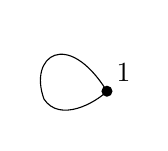
\begin{tikzpicture}[baseline=-2pt]\draw (0,0)..controls(-.5,.8)and(-1,.45)..(-.8,-.1)..controls(-.6,-.4)and(-.15,-.15)..(0,0);\fill (0,0) circle (2pt);\node[above right] at (0,0) {$1$};\end{tikzpicture}}
\end{array}}
\]
Il y a exactement un point à l'infini.

On a un morphisme (\uline{au dessus de} $\mathbf Z[\frac12]$)
\[
(78)\qquad \widehat M_{1,1}\longrightarrow\widehat M'_{\unsure{1,4|0,4}}\overset{\mathrm{déf}}=(\widehat M^!_{\unsure{1,4|0,4}},\mathfrak S_3)
\]
qui fait de $\widehat M_{1,1}$ une gerbe (de groupe constant $\{\pm1\}$) au dessus de $\widehat M'_{\unsure{1,4|0,4}}$ (en ca. $\neq2$) d'où
\[
[M_{1,1}]=\frac12[U_{0,3},\mathfrak S_3]=2[M_{0,4}]\deleted{\unsure{=\tfrac1{12}[\mathbf E^1]-\tfrac14}}\inserted{\unsure{T(1)}}
\]
\margin{62}
